  \documentclass[12pt]{exam}
\usepackage{amsthm}
\usepackage{libertine}
\usepackage[utf8]{inputenc}
\usepackage[margin=1in]{geometry}
\usepackage{amsmath,amssymb}
\usepackage{multicol}
\usepackage[shortlabels]{enumitem}
\usepackage{siunitx}
\usepackage{float}
\usepackage{cancel}
\usepackage{graphicx}
\usepackage{pgfplots}
\usepackage{listings}
\usepackage{tikz}


\pgfplotsset{width=10cm,compat=1.9}
\usepgfplotslibrary{external}
\tikzexternalize

\newcommand{\class}{Métodos Matemáticos} % This is the name of the course 
\newcommand{\examnum}{Examen Final} % This is the name of the assignment
\newcommand{\examdate}{\today} % This is the due date
\newcommand{\timelimit}{}
\newcommand{\Res}{\mathop{\mathrm{Res}}}





\begin{document}
\pagestyle{plain}
\thispagestyle{empty}

\noindent
\begin{tabular*}{\textwidth}{l @{\extracolsep{\fill}} r @{\extracolsep{6pt}} l}
	\textbf{\class} & \textbf{Name:} & \textit{Sergio Montoya}\\ %Your name here instead, obviously 
	\textbf{\examnum} &&\\
	\textbf{\examdate} &&
\end{tabular*}\\
\rule[2ex]{\textwidth}{2pt}
% ---

\begin{enumerate}
  \item \textbf{Teorema del Residuo}
    Primero, encuentra los polos de la función y su orden. Luego determina las singularidades dentro de la región que cierra la curva. Luego de eso aplica el teorema del residuo
    \begin{align*}
      \oint_{C} f\left( x \right) dx = 2\pi i \cdot \Res\left( f, \alpha \right) \\
    .\end{align*}
    El residuo puede valer:
    \begin{enumerate}
      \item Polo Simple: $\lim_{n \to z_0} \left( z - z_0 \right) f\left( z \right) $
      \item Polo de Orden $N$ : $\left[ \left( N - 1 \right)! \right]^{-1} \lim_{z \to z_0} \frac{d^{N - 1}}{dz^{N - 1}}\left( z - z_0 \right)^{N}d\left( z \right) $
    \end{enumerate}

    \begin{align*}
      f\left( z_0 \right) = \frac{1}{2\pi i}\int_C \frac{f\left( z \right) dz}{\left( z - z_0 \right) }\\
    .\end{align*}

  \item Delta de Dirac y Funciones de Green
    \begin{figure}[H]
      \centering
      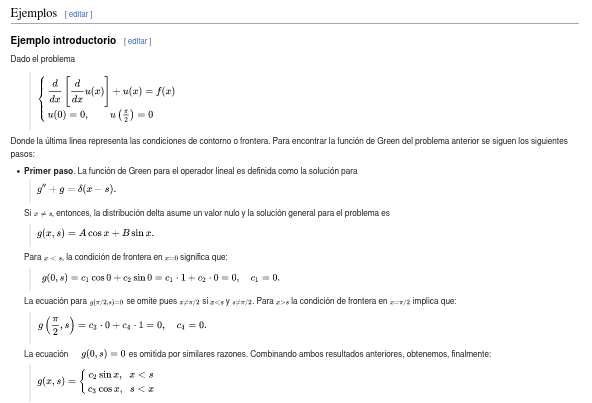
\includegraphics[width=0.8\textwidth]{green1.png}
      \caption{green1.png}
      \label{fig:green1-png}
    \end{figure}
    \begin{figure}[H]
      \centering
      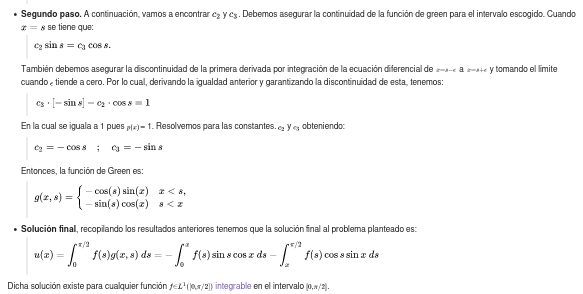
\includegraphics[width=0.8\textwidth]{green2.png}
      \caption{green2.png}
      \label{fig:green2-png}
    \end{figure}
  \item Parseval y seno y cose Fourier
    \begin{figure}[H]
      \centering
      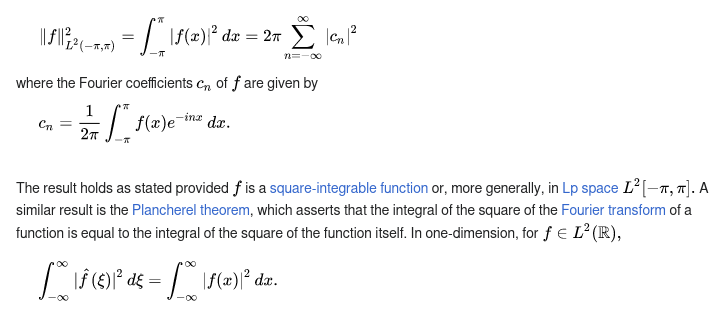
\includegraphics[width=0.8\textwidth]{parseval.png}
      \caption{parseval.png}
      \label{fig:parseval-png}
    \end{figure}
    \begin{figure}[H]
      \centering
      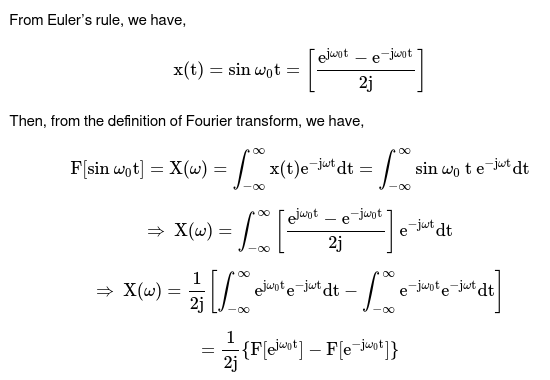
\includegraphics[width=0.8\textwidth]{sin1.png}
      \caption{sin1.png}
      \label{fig:sin1-png}
    \end{figure}
    \begin{figure}[H]
      \centering
      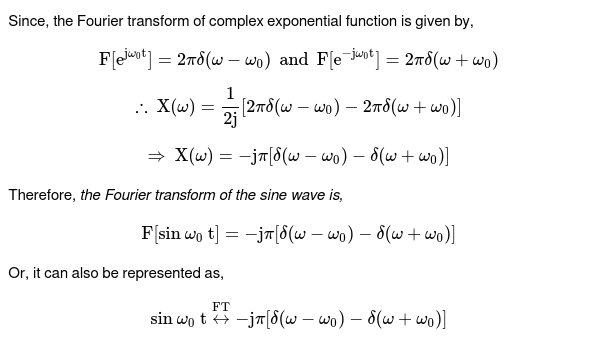
\includegraphics[width=0.8\textwidth]{sin2.png}
      \caption{sin2.png}
      \label{fig:sin2-png}
    \end{figure}
    \begin{figure}[H]
      \centering
      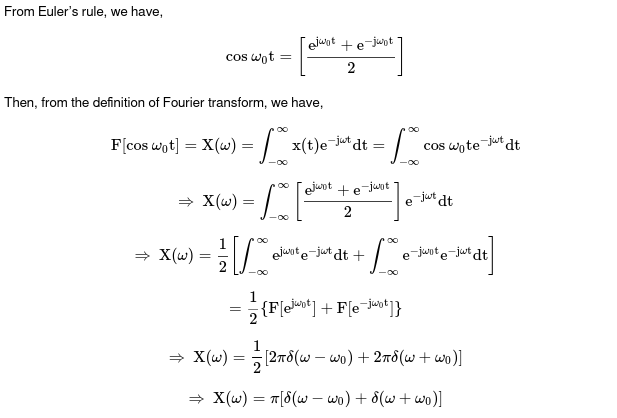
\includegraphics[width=0.8\textwidth]{cos1.png}
      \caption{cos1.png}
      \label{fig:cos1-png}
    \end{figure}
    \begin{figure}[H]
      \centering
      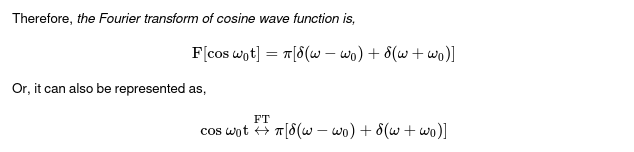
\includegraphics[width=0.8\textwidth]{cos2.png}
      \caption{cos2.png}
      \label{fig:cos2-png}
    \end{figure}
  \item Fourier
    \begin{figure}[H]
      \centering
      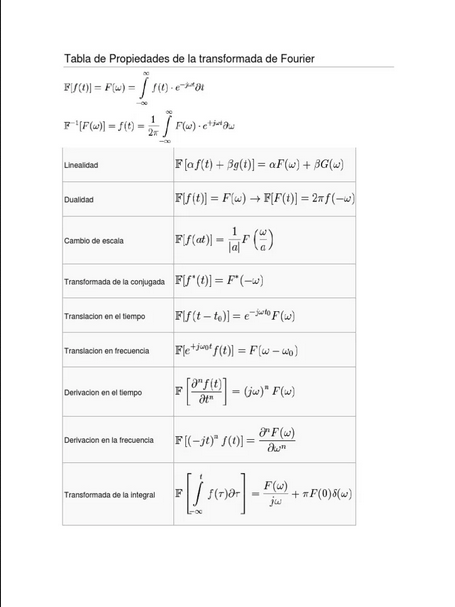
\includegraphics[width=0.8\textwidth]{fourier1.png}
      \caption{fourier1.png}
      \label{fig:fourier1-png}
    \end{figure}
  \item Laplace
    \begin{figure}[H]
      \centering
      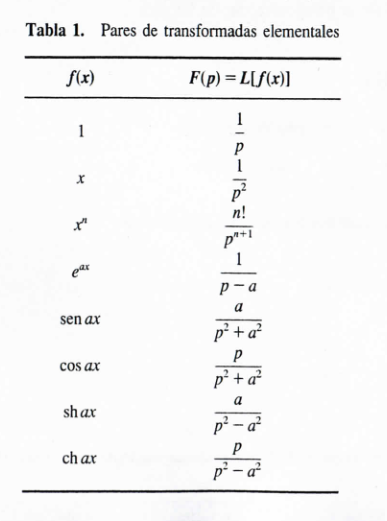
\includegraphics[width=0.8\textwidth]{laplace1.png}
      \caption{laplace1.png}
      \label{fig:laplace1-png}
    \end{figure}
    \begin{figure}[H]
      \centering
      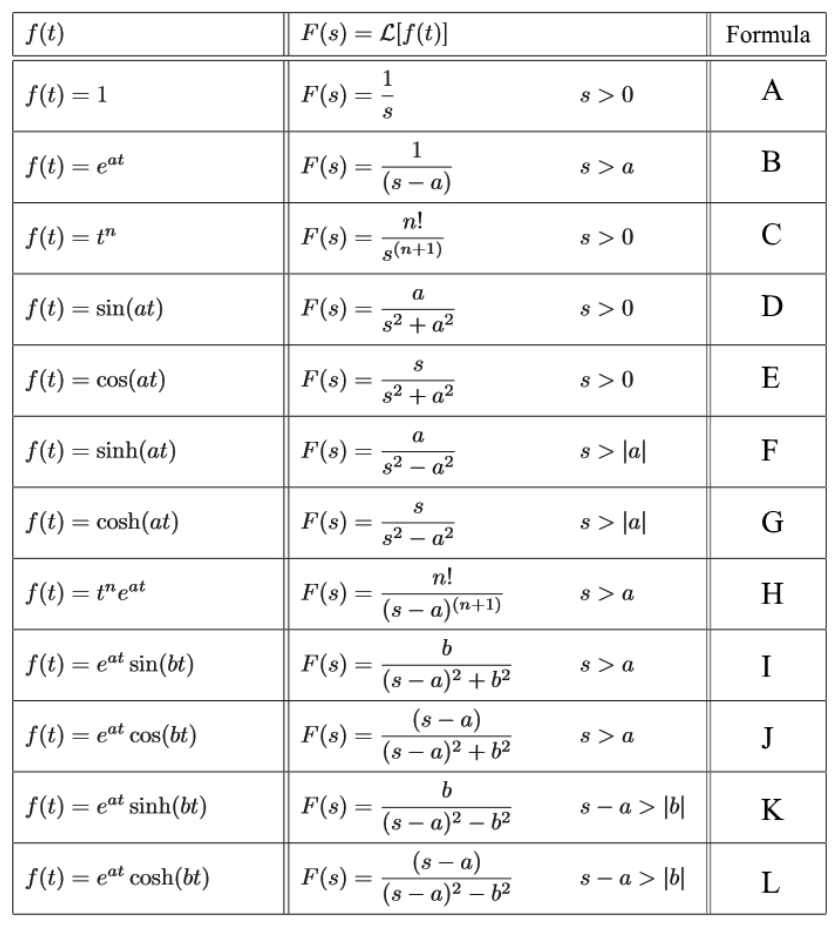
\includegraphics[width=0.8\textwidth]{laplace2.png}
      \caption{laplace2.png}
      \label{fig:laplace2-png}
    \end{figure}
  \item Funciones de Bessel
    \begin{figure}[H]
      \centering
      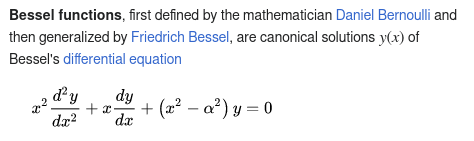
\includegraphics[width=0.8\textwidth]{bessel1.png}
      \caption{bessel1.png}
      \label{fig:bessel1-png}
    \end{figure}
    \begin{figure}[H]
      \centering
      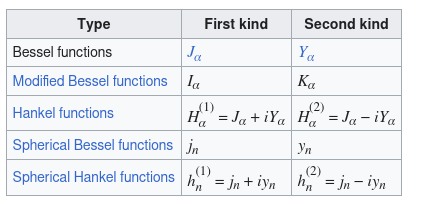
\includegraphics[width=0.8\textwidth]{bessel2.png}
      \caption{bessel1.png}
      \label{fig:bessel2-png}
    \end{figure}
    \begin{figure}[H]
      \centering
      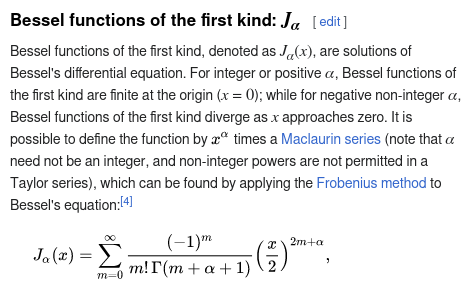
\includegraphics[width=0.8\textwidth]{bessel3.png}
      \caption{bessel1.png}
      \label{fig:bessel3-png}
    \end{figure}
    \begin{figure}[H]
      \centering
      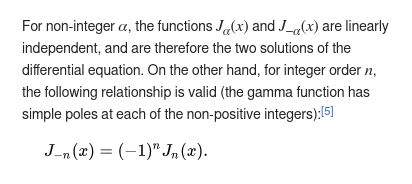
\includegraphics[width=0.8\textwidth]{bessel4.png}
      \caption{bessel1.png}
      \label{fig:bessel4-png}
    \end{figure}
    \begin{figure}[H]
      \centering
      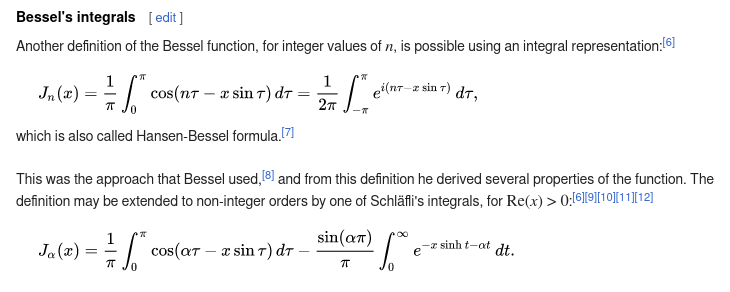
\includegraphics[width=0.8\textwidth]{bessel5.png}
      \caption{bessel1.png}
      \label{fig:bessel5-png}
    \end{figure}
    \begin{figure}[H]
      \centering
      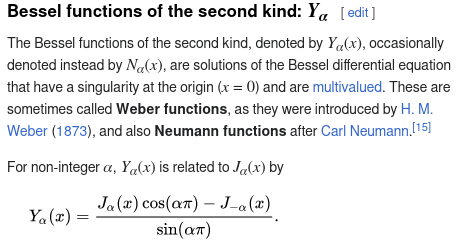
\includegraphics[width=0.8\textwidth]{bessel6.png}
      \caption{bessel1.png}
      \label{fig:bessel6-png}
    \end{figure}

    Ejemplo expansión de Bessel para $p^{(k)}$ :
        Suponemos que \[
    f\left( \rho \right) = \sum_{n=1}^{\infty} A_{v_n} J_v\left[ X_{v_n}\frac{\rho}{b} \right]
    .\] con
    \begin{align*}
      A_{v_n} &= \frac{2}{b^2\left[ J_{v + 1}\left( X_{v_n} \right) \right]^2}\int_{0}^{b}\rho\left( \rho^{k} \right) J_v\left( X_{v_n}\frac{\rho}{b} \right) d\rho\\
      \frac{d\left[ Y^{n}J_n \right] }{dy} &= Y^{n}J_{n - 1}\\
      A_{v_n} &= \frac{2}{b^2\left[ J_{v + 1}\left( X_{v_n} \right) \right]^2}\int_{0}^{b}\left( \rho^{k + 1} \right) J_v\left( X_{v_n}\frac{\rho}{b} \right) d\rho\\
      Y &= X_{v_n}\frac{\rho}{b} \\
      \frac{dY}{d\rho} &= \frac{X_{v_n}}{b} \leftrightarrow d\rho = \frac{b}{X_{v_n}} \\
      \rho &= \frac{Y b}{X_{v_n}} \\
      A_{v_n} &= \frac{2}{b^2\left[ J_{v + 1}\left( X_{v_n} \right)  \right]^2}\int_0^{X_{v_n}}\left( \frac{yb}{X_{v_n}} \right)^{k + 1}J_{v}\left( y \right) \frac{b}{x_{v_n}}dY\\
	      &= \frac{2}{b^2 \left[ J_{v+1}\left( X_{v_n} \right)  \right]^2}\int_{0}^{X_{v_n}}\frac{y^{k + 1}b^{k + 2}}{X_{v_n}^{k + 2}}J_v\left( Y \right) dY \\
	      &= \frac{2b^{k}}{\left[ J_{v+1}\left( X_{v_n} \right)  \right]^2 X_{v_n}^{(k + 2)} }\int_0^{X_{v_n}}Y^{k + 1}J_v\left( Y \right) dY \\
    \end{align*}
    Si $v = k$
    \begin{align*}
      \frac{d\left[ Y^{k}J_k\left( v \right)  \right] }{dY} &= Y^{k + 1}J_{k}\left( V \right)  \\
      A_{k_n} &= \frac{2b^{k}}{\left[ J_{v+1}\left( X_{v_n} \right)  \right]^2 X_{v_n}^{(k + 2)} }\int_0^{X_{v_n}}Y^{k + 1}J_v\left( Y \right) dY \\
      &= \frac{2b^{k}}{\left[ J_{v+1}\left( X_{v_n} \right)  \right]^2 X_{v_n}^{(k + 2)} }\left[ Y^{k}J_k\left( Y \right) \right]_0^{X_{k_n}}\\
      &=  \frac{2b^{k}}{\left[ J_{v+1}\left( X_{v_n} \right)  \right]^2 X_{v_n}^{(k + 2)} }  \left[ X_{k_n}^{k}J_k\left( x_{k_n} \right) - 0 \right] \\
      &= \frac{2b^{k}}{\left[ J_{v+1}\left( X_{v_n} \right)  \right]^2 X_{v_n}^{(k + 2)} } \frac{J_k\left( X_{k_n} \right) }{X^2_{k_n}} \\
      f\left( \rho \right) &= \rho^{k} = \sum_{n=1}^{\infty} \frac{2b^{k}}{\left[ J_{v+1}\left( X_{v_n} \right)  \right]^2 X_{v_n}^{(k + 2)} }\frac{J_k\left( X_{k_n} \right) }{X^2_{k_n}} J_k \left[ X_{k_n} \frac{\rho}{b} \right]
    .\end{align*}

  \item Laplace Ejemplo

          Tenemos la función: \[
	  f\left( x \right) =
      \begin{cases}
	V_0 &\ 0 < x \le 1\\
	-V_0 & -1 \le x < 0
      \end{cases}
      .\]
      Decimos entonces que la expresión de $f$ en polinomios de Legendre es: \[
      f\left( x \right) = \displaystyle \sum_{n=0}^{\infty} a_nP_n\left( x \right)
      .\] Donde los coeficientes están determinados por:
      \begin{align*}
	a_n &= \frac{2n + 1}{2} \int_{-1}^{1} f\left( x \right) P_n\left( x \right) dx \\
	    &= \frac{2n + 1}{2} \left[ \int_{-1}^{0} \left( -V_{0} \right) P_n dx + \int_{0}^{1}V_0P_n dx \right]\\
	    &= \frac{2n + 1}{2}V_0 \left[ \int_{0}^{1}P_n\left( x \right) dx - \int_{-1}^{0}P_n\left( x \right) dx \right]
      .\end{align*}

      Ahora bien, se tienen dos casos, $P_n$ par o impar:
      \begin{itemize}
        \item Para $P_n$ impar, $P_n\left( -x \right) = - P_n\left( x \right) \implies \int_{-1}^{0} P_n\left( x \right) dx = - \int_0^{1}P_n\left( x \right) dx$
	\item Para $P_n$ par, $P_n\left( -x \right) = P_n\left( x \right) \implies \int_{-1}^{0}P_n\left( x \right) dx = \int_0^{1} P_n\left( x \right) dx$
      \end{itemize}
      Con lo cual que podemos ver que los términos pares se contrarrestan. Por lo cual, tenemos que: \[
	a_n = \frac{2n + 1}{2}V_0 \left[ \int_0^{1}P_n\left( x \right) dx - \int_{-1}^{0}P_n\left( x \right) dx \right] = \left( 2n + 1 \right) V_0 \int_0^{1}P_n\left( x \right) dx
      .\] Luego: \[
      f\left( x \right)  = \sum_{n=0}^{\infty} \left( 2n + 1 \right) V_0 \int_{0}^{1}P_n\left( x \right) dx P_n\left( x \right)
      .\] Ademas, recordemos que $P_n$ es impar. Con esto entonces calculemos:
      \begin{align*}
	\int_{0}^{1} P_1 \left( x \right) dx &= \int_{0}^{1}x dx = \frac{x^2}{2} |_{0}^{1} = \frac{1}{2}\\
	\int_{0}^{1}P_3\left( x \right) dx &= \int_{0}^{1}\frac{1}{2}\left( 5x^{3}- 3x \right) dx\\
	&=  \frac{1}{2}\left[ \frac{5x^{4}}{4} - \frac{3x^2}{2} \right]_0^{1}\\
	&= \frac{1}{4}\left( \frac{5}{2} - 3 \right)  \\
	\implies& f\left( x \right) = \frac{3}{2}V_0 x - \frac{7}{8}V_0\left( 5x^{3}- 3x \right) + \ldots
      .\end{align*}


\end{enumerate}

\end{document}
